%%%%%%%%%%%%%%%%%%%%%%
%usenix
%\documentclass[letterpaper,twocolumn,10pt]{article}
%\usepackage{usenix2019,epsfig,endnotes}
%%%%%%%%%%%%%%%%%%%%%%
%CCS
\documentclass[sigconf]{acmart}

% remove reference format for submission
\settopmatter{printacmref=false}
%\settopmatter{printfolios=true}

% remove copyright box for submission
\renewcommand\footnotetextcopyrightpermission[1]{}

% control headers 
\fancyhf{} 
%\fancyhead[C]{Anonymous submission \#56 to ACM CCS 2019} % TODO: replace 9999 with your paper number
\fancyfoot[C]{\thepage}

\setcopyright{none} % No copyright notice required for submissions
%\acmConference[Anonymous Submission to ACM CCS 2019]{ACM Conference on Computer and Communications Security}{Due 5 February 2019}{London, UK}
%\acmYear{2019} 

%%%%%%%%%%%%%%%%%%%%%%
\usepackage{xcolor}
\usepackage{graphicx,pifont}
\usepackage{adjustbox}
\usepackage{caption}
\usepackage{subcaption}
\usepackage{mathtools}
\usepackage{mathrsfs}
\usepackage{xspace}
\usepackage{url}
\usepackage{tikz}
\usepackage{pifont}
\usetikzlibrary{positioning, trees, arrows, calc}
%\usepackage[font={small}]{caption}
%\usepackage{enumitem}
%\usepackage{cite}
%\usepackage{flushend}
%\usepackage{hyperref}
%\usepackage{caption}

\let\oldding\ding% Store old \ding in \oldding
\renewcommand{\ding}[2][1]{\scalebox{#1}{\oldding{#2}}}% Scale \oldding via optional argument

\newcommand{\zero}{\ding[1.2]{171}\xspace}
\newcommand{\one}{\ding[1.2]{172}\xspace}
\newcommand{\two}{\ding[1.2]{173}\xspace}
\newcommand{\three}{\ding[1.2]{174}\xspace}
\newcommand{\four}{\ding[1.2]{175}\xspace}
\newcommand{\five}{\ding[1.2]{176}\xspace}
\newcommand{\six}{\ding[1.2]{177}\xspace}
\newcommand{\seven}{\ding[1.2]{178}\xspace}
\newcommand{\eight}{\ding[1.2]{179}\xspace}
\newcommand{\nine}{\ding[1.2]{180}\xspace}
\newcommand{\ten}{\ding[1.2]{181}\xspace}

\newcommand*\circled[1]{\tikz[baseline=(char.base)]{
            \node[shape=circle,draw,inner sep=0.3pt] (char) {$#1$};}}

\newcommand{\blue}[1]{\textcolor{black}{#1}}
\newcommand{\red}[1]{\textcolor{red}{#1}}


\newcommand{\figsaver}[0]{\vspace{-5pt}}
\newcommand{\parasaver}[0]{\vspace{-2pt}}


\newif \ifremoveall
\removealltrue

\ifremoveall
\newcommand{\ad}[1]{\textcolor{red}{\textbf{Aritra: #1}}}
\newcommand{\ip}[1]{\textcolor{red}{Ivan: #1}}
\newcommand{\todo}[1]{\textcolor{red}{TODO: #1}}
\newcommand{\todoref}{\textcolor{red}{[ref]}}
\newcommand{\citneed}{[\textcolor{red}{cit}] }
\fi


\newcommand{\name}{\textsc{TrebucTee}\xspace}
\newcommand{\tool}{\textsc{\name API}\xspace}
\newcommand{\device}{\textsc{Device}\xspace}

\newcommand{\usb}{\texttt{USB}\xspace}
\newcommand{\tls}{\texttt{TLS}\xspace}


%%%%%%%%%%%%%%%%%%%%%%
%savetrees
%\usepackage[
%all=normal,floats=tight
%,paragraphs=tight
%,wordspacing=tight
%,mathspacing=tight
%,mathdisplays=tight
%]{savetrees}
%%%%%%%%%%%%%%%%%%%%%%

\newcommand{\myparagraph}[1]{\smallskip\noindent\textbf{#1.}\xspace}

%------------------------------------------------------------------------------
%                                Space savers.
%------------------------------------------------------------------------------
% This mylist environment indents items, and saves less space than the above.
\newcounter{myctr}
\newenvironment{mylist}{\begin{list}{\arabic{myctr}.}
{\usecounter{myctr}
\setlength{\topsep}{1mm}\setlength{\itemsep}{0.5mm}
\setlength{\parsep}{0.5mm}
\setlength{\itemindent}{1mm}\setlength{\partopsep}{0mm}
\setlength{\labelwidth}{-2mm}
\setlength{\leftmargin}{0mm}}}{\end{list}}

\newenvironment{mylist_indent}{\begin{list}{\arabic{myctr}.}
{\usecounter{myctr}
\setlength{\topsep}{1mm}\setlength{\itemsep}{0.5mm}
\setlength{\parsep}{0.5mm}
\setlength{\itemindent}{1.5mm}\setlength{\partopsep}{0mm}
\setlength{\labelwidth}{-2mm}
\setlength{\leftmargin}{0mm}}}{\end{list}}

% Space saving List environment for itemizing.
\newenvironment{mybullet}{\begin{list}{$\bullet$}
{\setlength{\topsep}{1mm}\setlength{\itemsep}{0.5mm}
\setlength{\parsep}{0.5mm}
\setlength{\itemindent}{0mm}\setlength{\partopsep}{0mm}
\setlength{\labelwidth}{-2mm}
\setlength{\leftmargin}{0mm}}}{\end{list}}


\graphicspath{{images/}}

\title{Dedicated Security Chips in the Age of Secure Enclaves} 

\author{Kari Kostiainen, Aritra Dhar, Srdjan Capkun \\ ETH Zurich}

\begin{document}
\maketitle
\thispagestyle{empty}

\begin{abstract}
\textbf{Secure enclave architectures have become prevalent in modern CPUs and enclaves provide a flexible way to implement various hardware-assisted security services. But special-purpose security chips can still have advantages. Interestingly, dedicated security chips can also assist enclaves and improve their security.}
\end{abstract}

\vspace{10pt}
\noindent
\textbf{Keywords ---} secure enclaves, security chips, trusted path, remote attestation, proximity verification


%\section*{}
\vspace{10pt}

Trusted Computing Base (TCB) minimization is one of the most fundamental computer security principles. The main idea is to reduce the amount of software and hardware that needs to be trusted for the secure operation of a particular application. A common technique to achieve TCB minimization is to run the application inside a Trusted Execution Environment (TEE). The TEE protects the application's execution, despite any other compromised software on the same system.

One TEE implementation approach that has gained significant popularity recently is to realize the TEE by enhancing the main CPU of the computing platform with new features like special instructions and access control checks. Intel's SGX, designed for the x86 architecture, is a prime example of such TEE. In SGX, the CPU ensures that no other process can access the memory of the protected application that is called an \emph{enclave}. By doing this, SGX guarantees that enclaves enjoy execution integrity, and their data remains confidential.  

Several other TEE designs exist too. ARM TrustZone is a popular TEE architecture that is used in many commercial mobile devices, while Sanctum~\cite{sanctum} serves as a good example of a research TEE system. For simplicity, we focus on Intel's SGX and use it as a case study to discuss the strengths and limitations of enclaves.

SGX-style enclaves are powerful security primitive. They are \emph{programmable}, and thus developers can implement almost arbitrary hardware-protected security services using them. This is in contrast to previous secure elements like TPMs that support only a fixed set of operations. Enclaves are also \emph{fast}, as they run on the main CPU of the computing platform, compared to significantly slower security elements like smart cards. And furthermore, enclaves are \emph{cheap}, since they require no additional hardware in contrast to expensive separate co-processors like HSMs. 

This combination of programmability, high performance, and low cost makes enclaves an attractive way to deploy various hardware-assisted security services. Indeed, after a decade of research and development into secure enclaves, the first large-scale commercial deployments are now starting. For example, Microsoft's Confidential Computing service uses SGX enclaves to protect customer data in the cloud.

The wide adoption of enclave architectures in modern CPUs is probably the most prominent trend in hardware-assisted security over the last decade. However, there is also another, more subtle trend appearing. Recently, computing service providers like Google and computer manufacturers like Apple have started to enhance their systems with special-purpose security chips. Google's cloud servers have a security chip called Titan in them~\cite{titan}, while Apple's computers come with the T2 security chip~\cite{t2}. 

At first glance, these two trends seem almost contradictory. If enclaves enable arbitrary hardware-protected security services, why do we still need dedicated security chips? 

In this article, we discuss the rationale behind this trend. We explain the benefits of dedicated security chips and outline two of our research projects where we designed such. These projects showcase an interesting new pattern --- one where special-purpose security chips assist enclaves and thus improve their security.

\section*{Dedicated Security Chips}

Computing platform providers have recently added new security chips to their systems. We look at two examples of this pattern: Google's Titan and Apple's T2 chips.

\subsubsection*{Google Titan}

Titan~\cite{titan} is a security chip implemented as a low-power microcontroller on Google's purpose-built server platforms. The Titan chip communicates with the main CPU via the Serial Peripheral Interface (SPI), and it interposes between the boot firmware flash and the Platform Controller Hub (PCH).

 One of the main functionalities that Titan implements is \emph{secure boot}. When the server machine is powered up, Titan executes code, known as boot ROM, from its embedded read-only memory. This code is immutable and thus implicitly trusted. The boot ROM code loads Titan's firmware from the embedded flash and verifies its integrity using a digital signature. Once Titan's firmware is securely verified and running, it can verify the boot process of its host. Titan blocks PCH's access to the firmware flash until it has cryptographically verified the content of the flash, and then it releases the lock and allows the verified boot firmware to configure the machine and load the boot loader which subsequently verifies and loads the OS. Such an iterative process allows precise control over which system software is booted. 

\begin{figure}[t]
    \centering
    \includegraphics[scale=0.7]{chips.pdf}
    \caption{Google Titan~\cite{titan} and Apple T2~\cite{t2} security chips.}
\label{fig:prototype}   
\end{figure}

 
\subsubsection*{Apple T2}
 
Apple's latest PCs come with a security chip called T2~\cite{t2} that also supports secure boot. When the machine with the T2 chip is turned on, T2 executes code from its read-only memory. This code verifies the next step of the T2's own boot process. Once T2 is fully running, it can verify the UEFI firmware, which will ensure that only authorized kernel will be booted on the host CPU.

Besides secure boot, T2 provides also other security features such as protecting the user's fingerprint values or making sure that the microphone is disconnected from the main CPU when the laptop's lid is closed. 
 
 
\subsubsection*{Missing Functionality}
  
Both Titan and T2 implement secure boot. Secure boot is also a good example of a security mechanism that cannot be implemented using SGX-style enclaves. 

In SGX, enclaves are constructed by the untrusted OS. The construction process of the enclave --- that is, the sequence of setup instructions and their parameters --- is recorded by the CPU so that it can be later communicated to an external verifier using the built-in attestation mechanism. This ensures that secrets will be provisioned only to correctly constructed enclave, and the untrusted OS cannot access those secrets. Thus, SGX enclaves are protected from the OS, but they \emph{cannot exist without it}. 

A direct implication of such TEE design is that enclaves cannot verify the integrity of the booted OS. (As noted in Textbox 1 above, other processor-based TEE architectures like the ARM TrustZone architecture are better suited for secure boot.) Because enclaves cannot implement all the needed security services, platform providers have added dedicated security chips, like Titan and T2, to implement the missing functionality. Disconnecting the microphones from the main CPU is another example of a security feature that cannot be implemented using enclaves.

%% ------------ %%

\begin{figure}
    \begin{tcolorbox}
    \textbf{Textbox 1:} 
    ARM TrustZone is a processor-based TEE architecture that is commonly used on smartphones. The main idea of TrustZone is to implement two separate execution modes on the main CPU. All untrusted software, like the OS and third-party apps, are executed in the \emph{normal world}, while applications that need protection run in a separate execution mode called the \emph{secure world}. The processor and memory controllers ensure that any process in the normal world cannot access the secure world.
    
    \hspace{10pt} TrustZone can enable secure boot~\cite{ekberg2014untapped}. A mobile device can be configured such that when the device is powered up, the main CPU starts executing implicitly trusted code that is loaded from read-only memory in secure world. This code can then verify the normal world boot loader before the CPU starts executing the main boot sequence of the normal world OS. Many smartphone manufacturers implement this approach.
	\end{tcolorbox}
\end{figure}  

%% ------------ %%

\subsubsection*{Security Weaknesses}

Besides missing functionality, enclaves also have security weaknesses. Since enclaves and untrusted code share the same CPU, they can be susceptible to side-channel leakage and microarchitectural attacks. The recently discovered Spectre and Meltdown vulnerabilities showed how transient execution could leak information across isolation boundaries. The same idea was successfully applied to extract secret keys from SGX enclaves in the Foreshadow attack~\cite{van2018foreshadow}. 

While specific attacks can be, and have been, mitigated (e.g., Intel's microcode updates include Spectre and Meltdown patches), side-channels and microarchitectural attacks continue to be a concern for enclaves. The root cause is that modern processors are extremely complex systems that have been optimized over decades. Enclave support was added on top of many layers of performance optimizations, and now, in hindsight, one can easily say that this approach was not the ideal foundation for strong isolation. In this regard, dedicated security chips have a clear advantage over enclaves.

Another security challenge is the rich interface between the untrusted OS and the enclave. Enclaves must interact with the operating system in many ways. For example, enclaves communicate by sending and receiving messages through the OS. Enclaves also need to safely pause their execution for interrupts. While enclave architectures provide coarse-grained memory isolation primitive at the hardware level, developers need to ensure that the interface is protected on the software level. Common implementation tasks include sanitization of buffers and safety checks for pointers. 

Because such checks are tedious, several enclave runtimes like the Open Enclave SDK have been developed to assist enclave developers. However, recent research has shown that many such enclave runtimes have classical memory safety vulnerabilities~\cite{van2019tale}. Because dedicated security chips do not need equally extensive interaction with the OS, the interface towards the untrusted OS is easier to protect tightly. 


\subsubsection*{Other Security Services?}

To summarize our discussion so far, enclaves cannot implement all useful platform security mechanisms, and they have significant security issues. Dedicated security chips can address both of these concerns. 

Obviously, the security services that can be implemented as dedicated security chips are not limited to the above-discussed examples. Which other services could be implemented as special-purpose security chips? 

Titan and T2 are integrated security chips that are permanently attached to the computing platform. Are there also use cases that would benefit from plug-and-play security tokens?

In the rest of this article, we explore these questions by examining two case studies from our recent research. Our first case is trusted path~\cite{protection}, \red{\#R1 where we explore how dedicated security chips enable trusted path to untrusted platform} and after that we focus on TEE identification and remote attestation~\cite{proximitee} \red{with a dedicated external hardware}.


\section*{Trusted Path}

SGX enclaves provide secure \emph{computation}, as their execution is isolated from other software on the same platform. However, they do not easily lend themselves to secure \emph{user interaction}. The main reason for this is that, in an architecture like SGX, enclaves communicate with I/O devices through the untrusted OS. When an enclave needs to receive user input, it is the responsibility of the OS to pass data from an input device like keyboard or mouse to the enclave. When an enclave needs to send user output, it is the responsibility of the OS to forward output data received from the enclave to a user output device like the screen. Such TEE design means that a compromised OS can easily modify any user input and output and read any secrets that are communicated between the user and the enclave. 

User input manipulation can have severe consequences in several application scenarios. For example, if a malicious OS modifies user input that is provided to a financial enclave, the enclave could be tricked to perform unauthorized payments. If enclaves are used to control safety-critical system such as a medical devices or industrial systems, user input modifications may cause serious safety risks. Also any enclave that needs to be configured with a password or similar user authentication credential is difficult to implement securely.

Such lack of secure user interaction capabilities means that enclaves do not support \emph{trusted path}~\cite{x86} --- a secure channel from the human user to the trusted application. 

%Depending on the application scenario, two different types of trusted paths may be desirable. The first, and more common, definition of trusted path is a secure communication channel between the human user and a \emph{local} trusted application like an enclave. The second, and perhaps less common, definition of trusted path is one that realizes a secure communication channel between the user and the \emph{remote} server without using any trusted local application in between. 


\subsubsection*{Design Principles}

Several projects have explored the idea of complementing commodity computing platforms with additional trusted hardware in an attempt to enable some form of a trusted path. While proposing extra hardware may be easy, the more difficult question becomes: what should the added hardware do to realize a trusted path? To answer this question, we look at noteworthy previous approaches. By examining their main limitations, we can identify general design principles for more secure trusted path.
	
The first approach that we look at is \textbf{transaction confirmation}~\cite{filyanov2011uni}. In such a solution, the user first completes the user interaction, such as payment, by interacting with the normal user interface of the untrusted platform. Once this is done, the user is expected to confirm his input, like a payment value and account number, using a separate hardware token, to detect and prevent any possible input value modifications.

This approach has two main problems. The first problem is that the user now has to interact with two separate user interfaces which reduces the usability of the solution significantly. The second, and more severe, problem is that such extra confirmation step is vulnerable to \emph{user habituation}, i.e, the possibility that user starts, after few successful transactions, confirming new payments without actually verifying their correctness. These observations lead us to the first design principle.  

\begin{tcolorbox}
\textbf{Principle 1:} Out-of-context security confirmations have high cognitive load and risk of user habituation. Thus, user interaction should be protected in the context of the normal user interface.
\end{tcolorbox}

The next known approach that we examine is \textbf{input trace signing}~\cite{IntegriKey}. Here, the main idea is to use a simple hardware device that sits \emph{in-between} a user input device, such as keyboard, and the untrusted computing platform. The device intercepts and signs every keypress, or similar user input event, and sends a signed trace to the trusted application. This approach is also known as ``bump-in-the-wire''~\cite{McCPerRei2006}. 

This approach meets our first principle, because the user does not have to perform additional security checks outside the main UI. However, such solutions are vulnerable to attacks, where the adversary manipulates user's input by showing false information on the output channel. One example of this is \emph{fake-typo} attack. Assume that the user types in value ``10'', but the adversary shows ``1'' on the screen. The user is likely to think that he mistyped and press ``0'' again. As a result, signed trace of ``100'' will be sent to the trusted application. This simple attack leads us to our next design principle.

\begin{tcolorbox}
\textbf{Principle 2:} User input and output integrity cannot be considered in isolation. Both must be protected simultaneously.
\end{tcolorbox}

The final approach that we examine is \textbf{secure overlays}. Fidelius~\cite{Fidelius} is an example system that follows this approach. FIdelius is based on two separate devices. One device intercepts keyboard presses and signs them for the trusted application, while another device intercepts the HDMI output signal and modifies it with secure overlays of security critical UIs such as payment web forms. 

Fidelius addresses the above mentioned problems, but is still vulnerable different type of user input manipulation that we call ``early-submission attack''. This attack is possible because Fidelius only protects keyboard input, but not mouse events. While this may seem only a functional limitation, it turns out that it is actually a security problem. Assume again, that the intention of the user is to submit value ``10''. Once user has typed ``1'', the untrusted computing platform generates a fake mouse event that submits the web form. Given this attack, we can state our last design principle.

\begin{tcolorbox}
\textbf{Principle 3:} All user input modalities must to be protected simultaneously.
\end{tcolorbox}


\subsubsection*{\protection System}

Given these principles, we designed new trusted path system called \protection. In the following, we focus on the use case where the trusted path is established between the user and a remote web server. That is, we want to protect interactions where the user completes and submits a security-critical web form. The same solution could be easily modified to create a trusted path between the user and a local enclave as well.

Figure~\ref{fig:architecture} shows the high-level architecture of \protection. The central component of the solution is a low-complexity embedded device called \hub that intercepts key presses from a keyboard and movement events from a mouse, tracks mouse movements, and draws secure overlays. 

\begin{figure}[t]
	\centering
	\includegraphics[trim={0 8.5cm 17cm 0}, clip, width=0.9\linewidth]{approachOverview.pdf}
	\caption{\protection architecture.}
	\label{fig:architecture}
\end{figure}

\begin{figure}[t]
	\centering
	\includegraphics[trim={0 8cm 15cm 0}, clip, width=\linewidth]{overlayScreenShot_new.pdf}
	\caption{\protection user interface.}
	\label{fig:screenshot}
\end{figure}

When the user visits a web page that contains a protected web form, the remote server sends a QR code to the user's platform, as shown in Figure~\ref{fig:screenshot} on the left. The QR code contains a specification of the security critical web form signed by the web server to prevent its modification by the untrusted browser and host platform. By using QR codes, we enable communication from the web server to the \hub device via an unmodified browser which makes deployment of this solution easy.

By examining the HDMI signal, \hub detects the QR code on the screen, decodes it and verifies its signature. After that, as is shown in Figure~\ref{fig:screenshot} in the middle, \hub renders the protected web form as an overlay on top of the HDMI frame that it receives from the host OS. This ensures that the security-critical UI elements are presented to the user as expected, and thus output integrity of the protected web form is preserved.

\hub tracks mouse movement events and when the mouse pointer enters the secure overlay, as shown in Figure~\ref{fig:screenshot} on the right, \hub dims the rest of the screen to focus the user's attention to the secure overlay. Such protection is needed to prevent the user from following fake mouse cursors drawn by the untrusted OS. Dimming parts of the screen has been shown to be an effective way to focus user's attention in the context of clickjacking studies~\cite{huang2012clickjacking}.

While the user interacts with the protected web form, \hub intercepts all input events. When the user clicks on the submit button, the \hub signs all inputs and sends them to the server via the untrusted browser. Since the submit button is part of the protected overlay and all mouse clicks are intercepted and signed by the \hub device, early-submission attacks are not possible. The server verifies the signed user inputs. 

If user input confidentiality is needed, the user cam be required to trigger a secure attention sequence (SAS), like \texttt{Ctr+Alt+Del}, before entering any secrets. The untrusted OS and the browser cannot observe sensitive data on the overlay, since they are rendered by \hub and never accessible to them.

The design of \protection complies with our design principles. Principle 1 is met, as the user only interacts with the main UI. Secure overlays support Principle 2 and mouse tracking combines with input trace signing makes sure that all input modalities are protected (Principle 3).

\begin{figure}[t]
	\centering
	\includegraphics[trim={0 6.6cm 21.5cm 0}, clip, scale=0.5]{setUp_1.pdf}
	\caption{\protection prototype.}
\label{fig:prototypeArch}   
\end{figure}

%\paragraph{Prototype} 
We implemented a fully-functional prototype of \protection which is shown in Figure~\ref{fig:prototypeArch}. The prototype includes a Raspberry Pi board as a computing unit, an Arduino board as input interceptor and a separate HDMI interceptor board. Such simple prototype shows that proposed functionalities are feasible to implement on low-cost hardware. Full details of the \protection system are explained in~\cite{protection}.

%The delay in forwarding keystrokes is $170\ \mu s$ and for frames is $21.76\ ms$. This allows the \protection to achieve the maximum display frame rate of $47.69$ per second (e.g., most of the movies are shot and shown in  ~24-30 fps)...






\section{Relay Attack on Intel SGX}

Trusted execution environments (TEEs) like Intel's SGX enable to securely execute applications on untrusted computing platforms. Remote attestation is a key feature of SGX, and other similar TEE architectures, as it allows a remote verifier to check that the attested enclave was correctly constructed before provisioning secrets to it. 

\begin{figure}[t]
 \centering
  %\includegraphics[trim={0 13.4cm 11cm 0},clip,width=\linewidth]{relayAttack.pdf}
  \includegraphics[trim={0cm 9cm 15.8cm 0},clip,width=0.75\linewidth]{relayAttack2.pdf}
 \caption{\textbf{Relay attack.} The adversary redirects attestation to his own platform which gives him increased (side-channel and kernel-level) abilities to attack the attested enclave.}
 \label{fig:SystemModel}
\end{figure}

\subsection{Relay Attacks}

We consider a system model shown in Figure~\ref{fig:SystemModel} that consists of three parties: the target platform, the remote verifier, and the attacker's platform. The remote verifier is a trusted party that wishes to connect and attest to a specific SGX platform. The target platform is the SGX platform to which the remote verifier intends to connect. Finally, the attacker's platform is a platform owned by the attacker that is connected to the target platform through the Internet.

\myparagraph{Adversary model.} We consider the following adversary model that we call the \emph{relay attacker}. The relay attacker controls the OS and all other privileged software on the \emph{target} platform at least \emph{temporarily}, in particular at the time of the remote attestation. The OS compromise on the target platform may be later detected and disinfected. We consider the case in which the target platform resides in a data center or otherwise in a facility with restricted physical access. The attacker hence \emph{does not} have physical access to the target platform (or any other co-located platform in the same facility).

The relay attacker controls the OS and all other privileged software on the attacker's platform \emph{permanently} and has physical access to that platform. The attacker also controls the network between the target platform and his platform. At the time of the attestation, the adversary has not been able to extract attestation or sealing keys from his platform or any other SGX processor.

\myparagraph{The relay attack.} The relay attacker can redirect the attestation requests intended for the target platform to his platform, as shown in Figure~\ref{fig:SystemModel}. This is a realistic attack for two reasons. First, in the SGX attacker's model the adversary is allowed to control the OS and can hence easily redirect any network request the target platform receives. Second, even if the attacker cannot compromise the OS in the target platform, it might be able to exploit some vulnerability of the untrusted application managing the enclave. The exploit might allow the attacker to manipulate the application's control flow to redirect attestation request to any platform he desires.


\begin{figure}[t]
\footnotesize
    \centering
    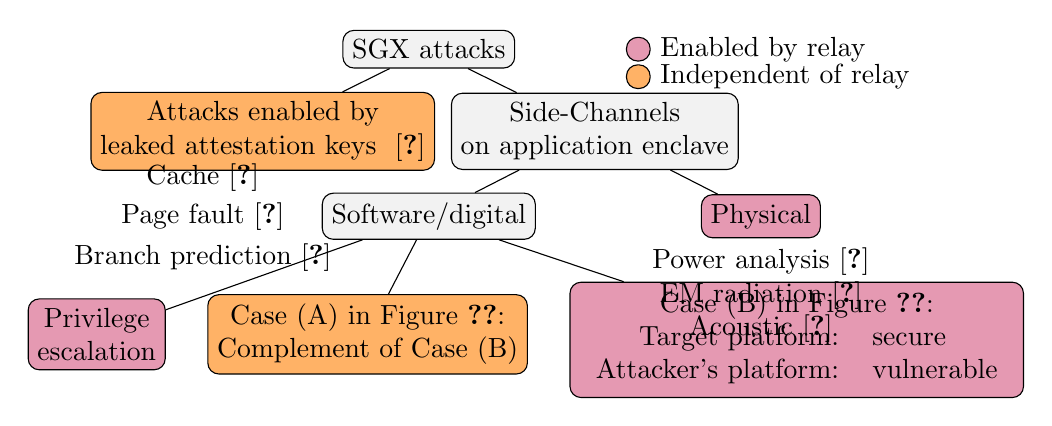
\begin{tikzpicture}[
solved/.style={rectangle,draw,fill=purple!40, rounded corners, align=center},
not/.style={rectangle, draw,fill=orange!60, rounded corners, align=center},
neutral/.style={rectangle, draw, rounded corners, align=center, fill=black!5},
sibling distance=12em]]
    \node[neutral](root) {SGX attacks}
    child { node[not, yshift=13pt] (name) {Attacks enabled by \\ leaked attestation keys ~\cite{foreshadow-usenix18}} }
    child { node[neutral, yshift=13pt] (app) {Side-Channels \\ on application enclave}
      child { node[neutral, yshift=12pt] (soft) {Software/digital}
		child { node[solved, yshift=0pt] (pe) {Privilege\\ escalation}}      
        child { node[not, right=1.5em of pe] (a) {Case (A) in Figure~\ref{fig:timeLine}:\\Complement of Case (B)}}
        child { node[solved, right=1.5em of a, yshift=-2pt] {Case (B) in Figure~\ref{fig:timeLine}:\\
            \begin{tabular}{rl}
                Target platform:& secure\\
                Attacker's platform:& vulnerable\\
            \end{tabular}}} }
      child { node[solved, yshift=12pt] (physical) {Physical} } };
      
    %\node[below=0cm of name] {Foreshadow~\cite{foreshadow-usenix18}};
    \node[below=0cm of physical](power) {Power analysis~\cite{wang2006covert}};
    \node[below=-5pt of power](EM) {EM radiation~\cite{gandolfi2001electromagnetic}};
    \node[below=-5pt of EM](ac) {Acoustic~\cite{shamir2004acoustic}};
         
    \node[left=10pt of soft](page) {Page fault~\cite{xu2015controlled}};
    \node[above=-3pt of page](cache) {Cache~\cite{dall2018cachequote}};
    \node[below=-2pt of page](branch) {Branch prediction~\cite{lee2017inferring}};
    %\node[below=-5pt of branch](synch) {Synchronization~\cite{asyncshock}};
      
    \node[solved, right=4em of root,  minimum size=3mm](l1) {};
    \node[right=0cm of l1](l1_1) {Enabled by relay};
    \node[not, below=1pt of l1, minimum size=3mm](l2) {};
    \node[right=0cm of l2](l2_1) {Independent of relay};
    
    \end{tikzpicture}
    
    \caption{\textbf{Relay attack implications.} The tree shows the types of attacks that are enabled by  redirection and ones that are independent of relay.}
    \label{fig:relayTree}
\end{figure}

            
\subsection{Relay Attack Implications}
\label{sec:problemStatement:implication}

Although relay attacks have been known for a long time~\cite{parno2008bootstrapping}, their implications to modern TEEs like SGX have not been carefully analyzed. Next, we perform the first such analysis.

The main consequence of attestation redirection is that it \emph{increases the adversary's ability to attack the attested enclave} through side-channels which are a well-known limitation of SGX (see Section~\ref{sec:background:attacks}). In Figure~\ref{fig:relayTree} we highlight two major classes of attacks: those that are only possible by first performing a relay attack, which we denote as ``enabled by relay'', and those that can be done whether or not the attacker also does a relay attack, which we call ``independent of relay.''

\myparagraph{Attacks using leaked attestation keys.}
Our first observation is that attacks based on leaked attestation keys (e.g., ones obtained through the Foreshadow attack~\cite{foreshadow-usenix18}) are independent of relaying. If the adversary has obtained a valid and non-revoked attestation key, he can emulate an SGX processor on the target platform and obtain any secrets provisioned to it. %We revisit such emulation attacks and propose a solution for addressing them in Appendix~\ref{sec:variantII}. 

\myparagraph{Physical side channels.}
One major benefit of the relay, from the adversary's point of view, is that it enables \emph{physical} side-channel attacks against application enclaves. Once a secret has been provisioned to the attacker's platform, she has as much time as she likes to perform the attack. Some examples of physical side-channel attacks are acoustic, electric and electromagnetic monitoring, which have been shown to be both effective and inexpensive means to extract secrets from modern PC platforms . Since the adversary does not have physical access to the target platform, such attacks are clearly not possible without relay. Hardening programs like enclaves against physical side channels is difficult and currently an open problem. Therefore, developers cannot easily defend their enclaves against physical side channels that are enabled by attestation redirection.

\myparagraph{Privilege escalation for digital side channels.}
Another possible benefit of relay attacks is that it may enable \emph{privilege escalation}. In cases where the adversary has only compromised the user-space application that manages the enclave, and not the OS, the application can redirect the attestation to the attacker's remote platform where he controls the OS as well. In such cases, the relay enables \emph{digital} side-channel attacks that require system privileges.

\iffalse
\begin{figure}[t]
\footnotesize
    \centering
    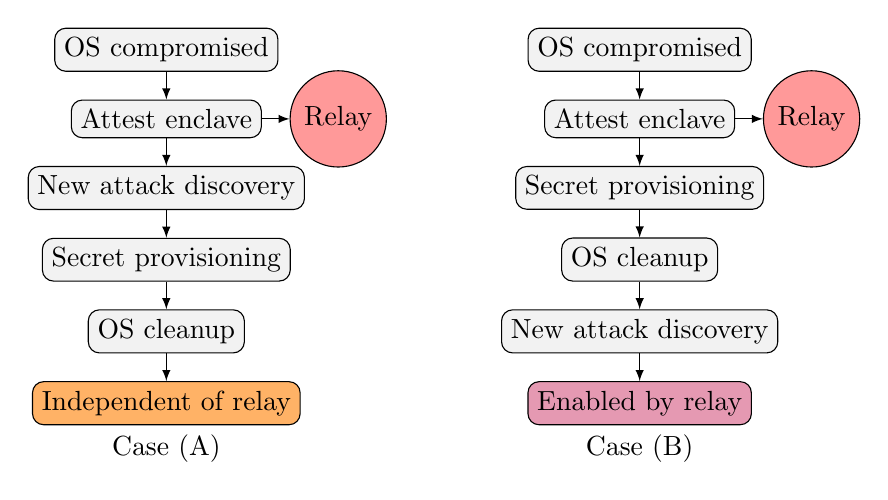
\begin{tikzpicture}[
    solved/.style={rectangle,draw,fill=purple!40, rounded corners, align=center},
    relayNode/.style={circle,draw,fill=red!40, align=center},
    edge from parent/.style={draw,-latex},    
    neutral/.style={rectangle, draw, rounded corners, align=center, fill=black!5},
    not/.style={rectangle, draw,fill=orange!60, rounded corners, align=center},
    sibling distance=12em]]
    
        
  \node[neutral](root1) {OS compromised}
        child { node[neutral, below = 1em of root1] (attestation1) {Attest enclave}     
         child { node[relayNode, right = 1em of attestation1] (relay1) {Relay}}
            child { node[neutral, below = 1em of attestation1] (discovery1) {New attack discovery}
                child { node[neutral, below = 1em of discovery1] (provisioning1) {Secret provisioning}     
                        child { node[neutral, below = 1em of provisioning1] (cleanup1) {OS cleanup} 
                            child { node[not, below = 1em of cleanup1] (attack1) {Independent of relay}  } } } } };  
            
   \node[below=0cm of attack1] {Case (A)};
 
 
  \node[neutral, right = 9em of root1](root) {OS compromised}
        child { node[neutral, below = 1em of root] (attestation) {Attest enclave}     
         child { node[relayNode, right = 1em of attestation] (relay) {Relay}}
             child { node[neutral, below = 1em of attestation] (provisioning) {Secret provisioning} 
                child { node[neutral, below = 1em of provisioning] (cleanup) {OS cleanup}
                child { node[neutral, below = 1em of cleanup] (discovery) {New attack discovery}                 
                            child { node[solved, below = 1em of discovery] (attack) {Enabled by relay}  } } } } };  
                
    \node[below=0cm of attack] {Case (B)};
    
    
    \end{tikzpicture}
    \caption{Example sequences of events where attestation redirection either enables digital side-channel attacks (B) or where the attack success is independent of relay (A). \todo{This figure should be improved. Where is the secret provisioned and at which time is all that matters. But this info is not clearly conveyed in the picture.}} 
    \figsaver
    \label{fig:timeLine}
\end{figure}
\fi

\begin{figure}[t]
\footnotesize
    \centering
    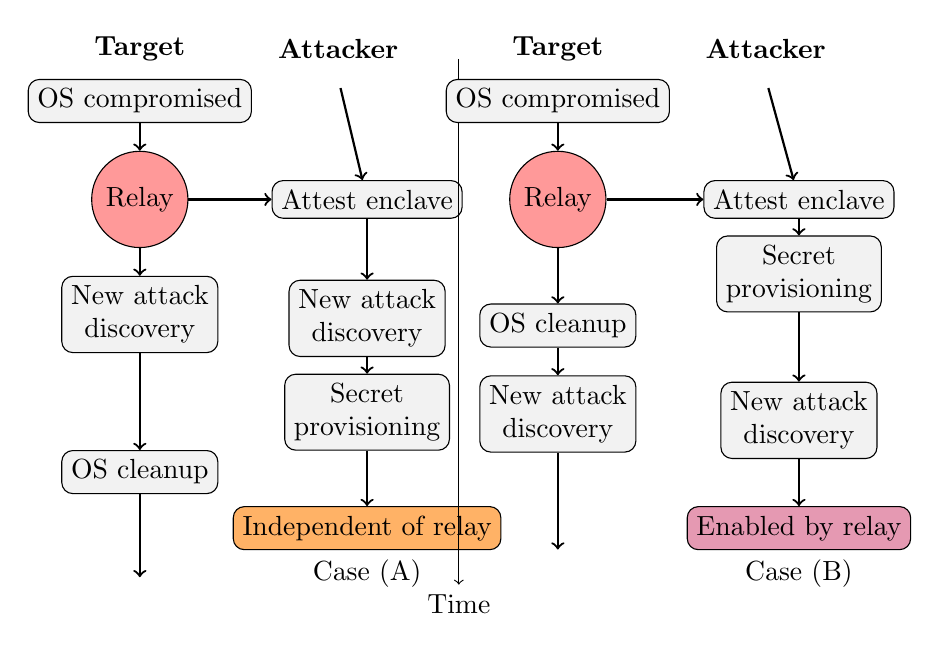
\begin{tikzpicture}[
    solved/.style={rectangle,draw,fill=purple!40, rounded corners, align=center},
    relayNode/.style={circle,draw,fill=red!40, align=center},
    edge from parent/.style={draw,-latex},    
    neutral/.style={rectangle, draw, rounded corners, align=center, fill=black!5},
    not/.style={rectangle, draw,fill=orange!60, rounded corners, align=center},
    sibling distance=12em]]
    
 
 
 \node[] (targetA) {\textbf{Target}};
 \node[right=0.93cm of targetA] (attackA) {\textbf{Attacker}};
 \node[below=0 of attackA] (dummy) {};
 
  
 \node[neutral, below=0.1cm of targetA](root1) {OS compromised};    
 \node[relayNode, below = 1em of root1] (relay1) {Relay};
 \node[neutral, right = 3em of relay1] (attestation1) {Attest enclave};
 \node[neutral, below = 1em of relay1] (discovery1) {New attack\\ discovery};        
  \node[neutral, below = 2.2em of attestation1] (discoveryAttack1) {New attack\\ discovery};  
 \node[neutral, below = 0.6em of discoveryAttack1] (provisioning1) {Secret\\ provisioning};
 \node[neutral, below = 3.5em of discovery1] (cleanup1) {OS cleanup};    
 \node[below = 3em of cleanup1] (end) {};      
 \node[not, below = 2em of provisioning1] (independent) {Independent of relay}; 
 
 
  \draw[->, thick] (root1) edge[] node{} (relay1);
 \draw[->, thick] (relay1) edge[] node{} (discovery1);
 \draw[->, thick] (relay1) edge[] node{} (attestation1);
 \draw[->, thick] (attestation1) edge[] node{} (discoveryAttack1);
 \draw[->, thick] (discovery1) edge[] node{} (cleanup1); 
 \draw[->, thick] (discoveryAttack1) edge[] node{} (provisioning1);
 \draw[->, thick] (provisioning1) edge[] node{} (independent);
 \draw[->, thick] (dummy) edge[] node{} (attestation1);
 \draw[->, thick] (cleanup1) edge[] node{} (end);
  \node[below=0cm of independent] {Case (A)};
 

 \node[right=0.52cm of attackA](point1){};
 \node[below=19em of point1](point2){Time};
 \draw[->] (point1) edge[] node{} (point2);
 
 \node[right=1.2cm of attackA] (targetB) {\textbf{Target}};
 \node[right=1.05cm of targetB] (attackB) {\textbf{Attacker}};
  \node[below=0 of attackB] (dummy1) {};
 
 %\draw ($(attackA)!0.5!(targetB)$) -- ($(attackA)!0.5!(targetB) - (0, 5)$);    
 \node[neutral, below=0.1cm of targetB](root) {OS compromised};
 \node[relayNode, below = 1em of root] (relay) {Relay};
 \node[neutral, right = 3.5em of relay] (attestation) {Attest enclave};
 \node[neutral, below = 0.6em of attestation] (provisioning) {Secret\\ provisioning};
 \node[neutral, below = 2em of relay] (cleanup) {OS cleanup};
 \node[neutral, below = 1em of cleanup] (discovery) {New attack\\ discovery};   
 \node[below = 3.5em of discovery] (end1) {};        
 \node[neutral, below = 2.5em of provisioning] (discoveryAttack) {New attack\\ discovery};           
 \node[solved, below = 1.7em of discoveryAttack] (attack) {Enabled by relay}; 
 
 
 \draw[->, thick] (root) edge[] node{} (relay);
 \draw[->, thick] (cleanup) edge[] node{} (discovery); 
 \draw[->, thick] (discoveryAttack) edge[] node{} (attack);
 \draw[->, thick] (relay) edge[] node{} (cleanup);  
 \draw[->, thick] (provisioning) edge[] node{} (discoveryAttack); 
 \draw[->, thick] (relay) edge[] node{} (attestation);
 \draw[->, thick] (attestation) edge[] node{} (provisioning);        
 \draw[->, thick] (dummy1) edge[] node{} (attestation);
 \draw[->, thick] (discovery) edge[] node{} (end1);
\node[below=0cm of attack] {Case (B)};
   

                         
    \end{tikzpicture}
    \caption{Example sequences of events. In Case A the attack success is independent of relay. In Case B attestation redirection enables the attack.} 
    \label{fig:timeLine}
\end{figure}


\myparagraph{Attacks that depend on timing of events.}    
The third, and perhaps the most subtle, implication of relay is that it can also enable software-based side-channel attacks that would not be possible to launch on the target platform due to \emph{timing of certain events}. These events include, but are not restricted to the provisioning of secrets to the enclave, the possible disinfection of the target platform from malicious software, and the discovery of a new side-channel attack. 

We group the relative ordering of these events into two cases: A and B. Case A covers event sequences that only lead to attacks which are independent of relay and Case B covers event sequences in which redirection gives extra capabilities to the adversary. Below, and in Figure~\ref{fig:timeLine}, we provide examples of sequences belonging to these two cases:

\begin{mylist}
    \item[\emph{Case A: independent of relay.}] A digital side-channel is independent of relay if the adversary could perform it on the target platform as well. An example of such case is shown th timeline depicted in Figure~\ref{fig:timeLine}, where a new attack is discovered after secret provisioning but before the target platform OS is disinfected.
    
    %If the vulnerability was discovered before the secret provisioning, we could assume that the enclave developers patched these vulnerabilities in the code. Hence attacker cannot execute the side channel attack after the relay. However, in case the developers did not publish the patched version of the enclave code before the provisioning of the secret to the enclave, the attacker can still execute relay attack and the extract the secret from his platform.

    \item[\emph{Case B: attack enabled by relay.}] Case B is reached whenever it occurs that by using a side channel the enclave is exploitable on the attacker's platform, but not on the target platform. 
    %In this case, by having the foresight to provision the enclave on its platform, the attacker has the possibility to launch an attack on an enclave that would otherwise be secure on the target platform. 
    A timeline of such case is shown in Figure~\ref{fig:timeLine}, where at the time of attestation and secret provisioning, the enclave is hardened against all known digital side-channel attacks (using tools like Raccoon~\cite{raccoon}). After secret provisioning, the OS compromise is detected and cleaned. Later, a new side-channel attack vector (that is not prevented by the used tools) is discovered. If the adversary performed redirection and the secret was provisioned to the attacker's machine, the new side channel is exploitable. Without the relay, the attack is not possible.
    
    %If the vulnerability is discovered after the secret provisioning, that attacker will have some time on this platform (relayed) where the unpatched enclave code runs before the software patch takes place.} 
\end{mylist}

\section*{Deployment Options and Security Benefits}

Now that we have seen two commercially deployed, integrated security chips (Titan and T2) and another two research projects where we designed user-attachable dedicated security tokens (\protection and \proximitee), we can compare these solutions based on their deployment options and security benefits. 

\paragraph{Deployment}
Integrated security chips like Titan or T2 can be only issued by major service and platform providers that have the possibility to design and build their own systems. 

\proximitee is an example of a plug-and-play security token that can be attached to the target platform over a standard interface like USB. Obviously, the deployment of security solutions is a feasible option for a larger set of service providers. For example, cloud computing providers can enhance off-the-shelf servers with \proximitee tokens to enable secure, relay-protected attestation on them. Another interesting use case is the secure setup of a permissioned blockchain where every consensus node is hardened with SGX enclaves. The trusted authority that appoints the consensus nodes and bootstraps the chain can issue a \key token to each organization that operates one node.

Also \protection could be deployed as a plug-and-play security module. A user-pluggable token is a good deployment option for web-based online services like e-voting and online banking. Such deployment allows voting authorities and banks to increase the security of their services without restricting the users’ choice of client platform. In medical and industrial domains, an externally-attached \protection module can improve the security of safety-critical systems, even when modifications to the computing platform itself are prohibited due to strict regulations. Alternatively, \protection could be deployed as an integrated security chip such that its functionality is implemented as part of the integrated keyboard, mouse, and display controllers of the computing platform. 

%\begin{figure}[t]
%    \centering
%    \includegraphics[scale=0.4]{comparison.pdf}
%    \caption{Comparison of \protection and \proximitee with respect to the platform-integrated security chips, user-pluggable security tokens and CPU-implemented enclave architecture.}
%\label{fig:prototype}   
%\end{figure}

\paragraph{Security Benefits}
Titan and T2 are chips that enable security functionality like a secure boot that is missing from enclaves. Thus, the operation of Titan and T2 is largely orthogonal to the operation of enclaves. 

In comparison, \proximitee is a security chip that is designed to work in collaboration with enclaves and improve their security guarantees by enabling secure TEE identification for hardened remote attestation. 

\protection is a solution that can either assist enclaves or operate independently of them. One possible usage for \protection is to enable a trusted path from the user to a local enclave, which can, in turn, can communicate securely with remote servers. In such a deployment, \protection works in collaboration with an enclave and addresses one of the limitations of the SGX architecture --- it's lack of trusted path. Alternatively, \protection could be used to create a trusted path from the user to a remote server without the use of enclaves. Such a deployment option may be beneficial, for example, in cases where the risk of microarchitectural attacks on enclaves is considered too high, and thus, the integrity of the trusted path should not rely on enclave security.




\section*{Outlook}

%We end this article by outlining possible future directions for enclaves and dedicated security chips. We also discuss how these two closely-related but still somewhat different hardware-assisted security mechanisms can work in collaboration.

%Future computing architectures are likely to be more diverse than the ones we use today. The paradigm that has been prevalent for the past few decades is to perform most of the computation in one or more general-purpose processing units. Modern computing platforms often incorporate more specialized computing units like GPUs. 

Future computing platforms will combine various computing units like CPUs, GPUs, TPUs, FPGAs and more. %~\cite{dean2018new}.
Similar to the current enclave architectures that enhance CPUS with secure execution, also the other processing units like GPUs and FPGAs will need secure computation. There are already several on-going research efforts that explore the design of such TEEs~\cite{volos2018graviton}.

Our research on trusted path (the \protection system) highlights that I/O devices need secure communication with enclaves. Similarly, also other peripherals like GPS units and fingerprint sensors would benefit from secure communication with enclaves. Protected communication between TEEs and other platform components requires secure authentication, enclave identification and access control mechanisms. The ARM TrustZone architecture has limited support towards this direction. In TrustZone, hardware components like memory controllers can make coarse-grained access control decisions based on the CPU's execution mode~\cite{ekberg2014untapped}. 

%However, this approach lacks the possibility of distinguishing one enclave from another. Such intra-platform communication is also not secure against simple physical attacks like bus tapping. 

Extending this paradigm for more fine-grained access control and strongly-secured inter-component communication is one promising future direction. We envision future computing platforms where enclaves, peripherals and special-purpose security chips all work together to provide a rich set of hardware-assisted platform security services.


{\small
\bibliographystyle{abbrv}
\bibliography{references}}
 


\section*{Author bios}

\begin{tcolorbox}

\paragraph{Kari Kostiainen} is a Senior Scientist at ETH Zurich. His research interests include trusted computing, mobile security, secure user interaction and blockchain security. Dr. Kostiainen has a PhD degree from Aalto University. His contact address is \emph{kari.kostiainen@inf.ethz.ch}.

\vspace{10pt}
\paragraph{Aritra Dhar} is a PhD Student at ETH Zurich. His research interests include secure user interaction, trusted computing, anonymous networks and program analysis. Mr. Dhar has a master's degree from IIIT Delhi. His contact address is \emph{aritra.dhar@inf.ethz.ch}.

\vspace{10pt}
\paragraph{Srdjan Capkun} is a Full Professor at ETH Zurich. His research interests include wireless security, secure positioning, trusted computing and blockchain technologies. Prof. Capkun has a PhD degree from EPFL and he is an ACM Fellow. His contact address is \emph{srdjan.capkun@inf.ethz.ch}.

\end{tcolorbox}
 
 
\end{document}
